\documentclass[11pt]{report}

\usepackage{dirtree}
\usepackage{graphicx}

\author{Xinyu Tian, Zesen Zhuang}
\date{\today}
\title{Project 3 Report}

\begin{document}
\maketitle

\setlength{\parindent}{0em}
\setlength{\parskip}{0.3em}

\section{Project Structure}

\dirtree{%
.1 .
.2 dashboard \DTcomment{dashboard source code for task 2}.
.3 Dockerfile.
.3 app.py.
.3 data.json.
.3 requirements.txt.
.3 utils.
.4 helper\_functions.py.
.3 wsgi.py.
.2 k8s \DTcomment{kubernetes configurations for task 1, 2, 3}.
.3 base \DTcomment{using provided serverless runtime, task 1, 2}.
.4 kustomization.yaml.
.4 outputkey-config.yaml.
.4 pyfile-config.yaml.
.4 serverless-deployment-course.yaml.
.3 overlays.
.4 dev \DTcomment{Using implemented serverless runtime, task 3}.
.5 deployment.yaml.
.5 kustomization.yaml.
.5 pyfile.
.5 service.yaml.
.3 pyfile-config.yaml.
.2 makefile.
.2 ourmodule.py \DTcomment{usermodule for task 1}.
.2 requirements.txt.
.2 serverless-runtime \DTcomment{serverless runtime source code for task 3}.
.3 Dockerfile.
.3 main.py.
.3 requirements.txt.
.3 tests.
.4 test\_redis\_connection.py.
.3 usermodule\_dumour.py.
.3 utils.
.4 context.py.
.4 redis\_connection.py.
}

The project structure is shown in the above tree which illustrates the code to submit for each task.

\section{Compatibility}

In Task 3, our implementation of the serverless runtime observed good compatiblity with the provided serverless runtime. 

\begin{enumerate}
    \item The serverless runtime can be deployed to the Kubernetes cluster and the user module can be invoked by the serverless runtime.
    \item We did not need to change the user module to make it compatible with the new serverless runtime.
    \item We added more error handling, such as logging debug info and throwing errors mechanisms to the serverless runtime to make it more robust.
    \item Another difference between our implementation and the provided ser-verless runtime is that we execute the handler function more frequently.
    \item We did not need to change the dashboard code to make it compatible with the new serverless runtime. we tested both the bare and containerized version of the dashboard and they both runs well.
\end{enumerate}

\newpage

\section{Dashboard}

Our dashboard monitors 4 different metrics: CPUs usage, virtual memory usage, CPU frequency, and number of processes.

\begin{figure}[!htbp]
    \centering
    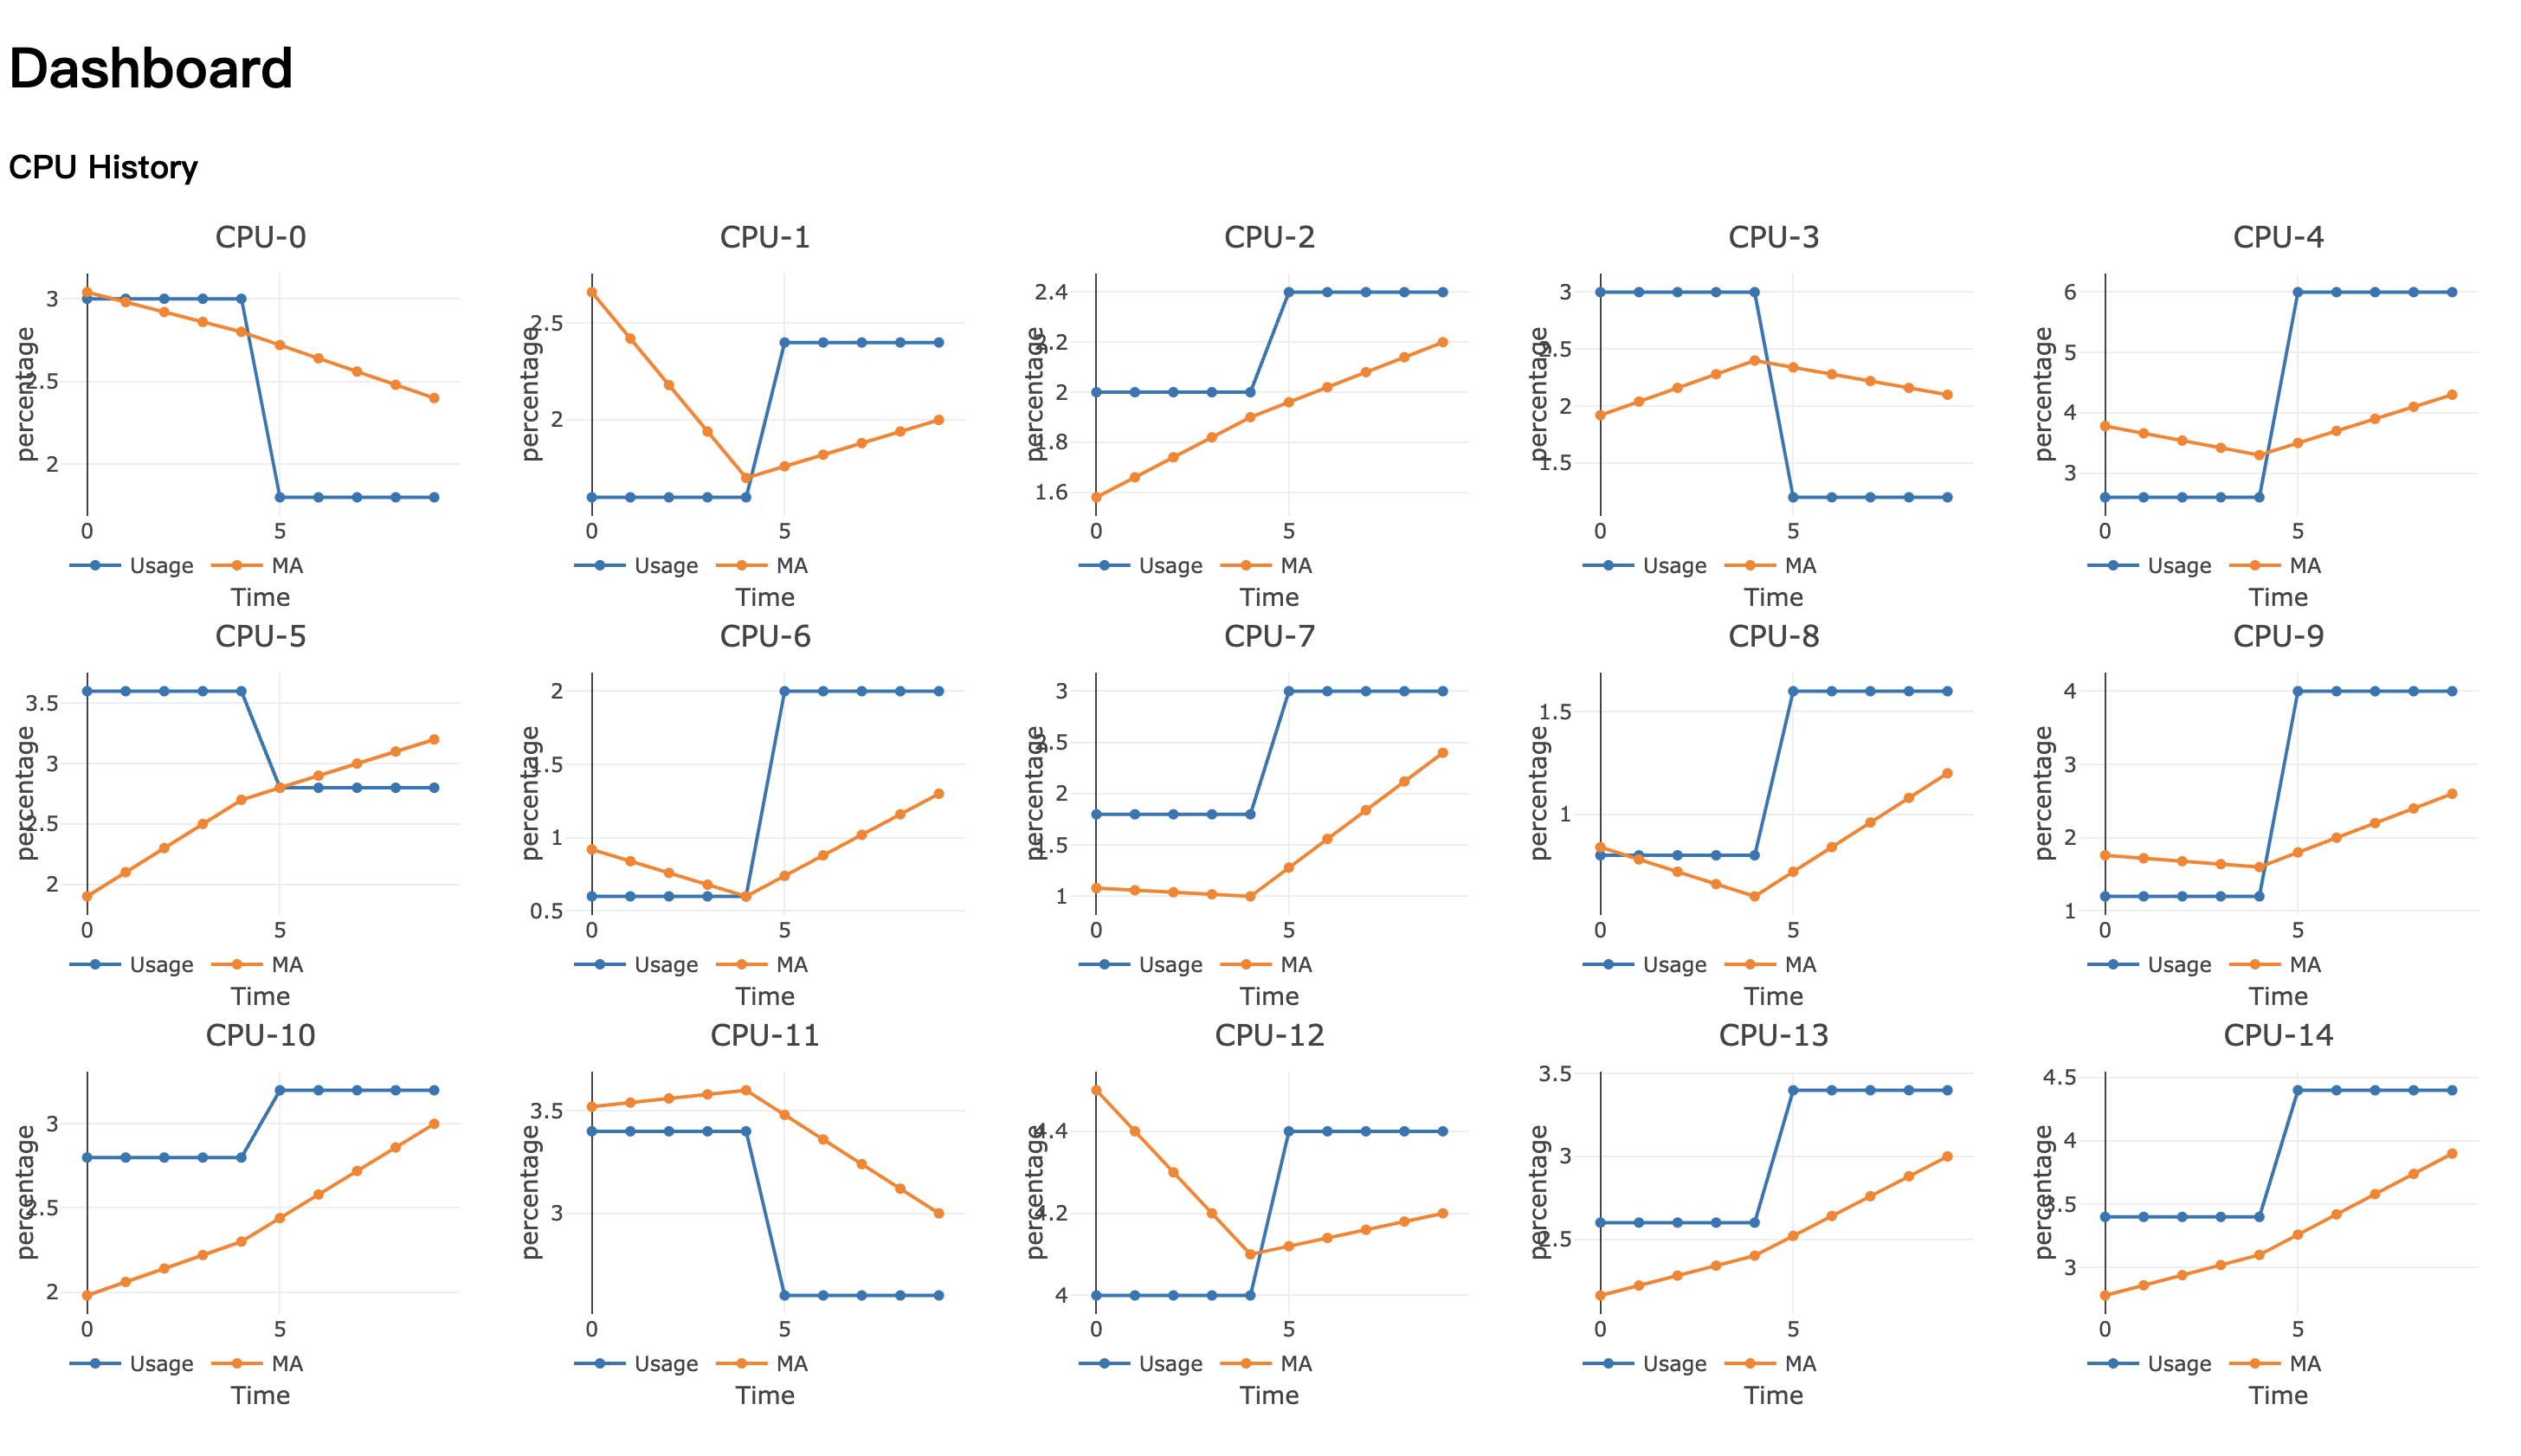
\includegraphics[width=0.95\textwidth]{figures/cpu-usage.png}
    \caption{CPU Usage}
    \label{fig:cpu-usage}
\end{figure}

Figure \ref{fig:cpu-usage} shows the visualization of history and moving average of CPU usages.

\begin{figure}[!htbp]
    \centering
    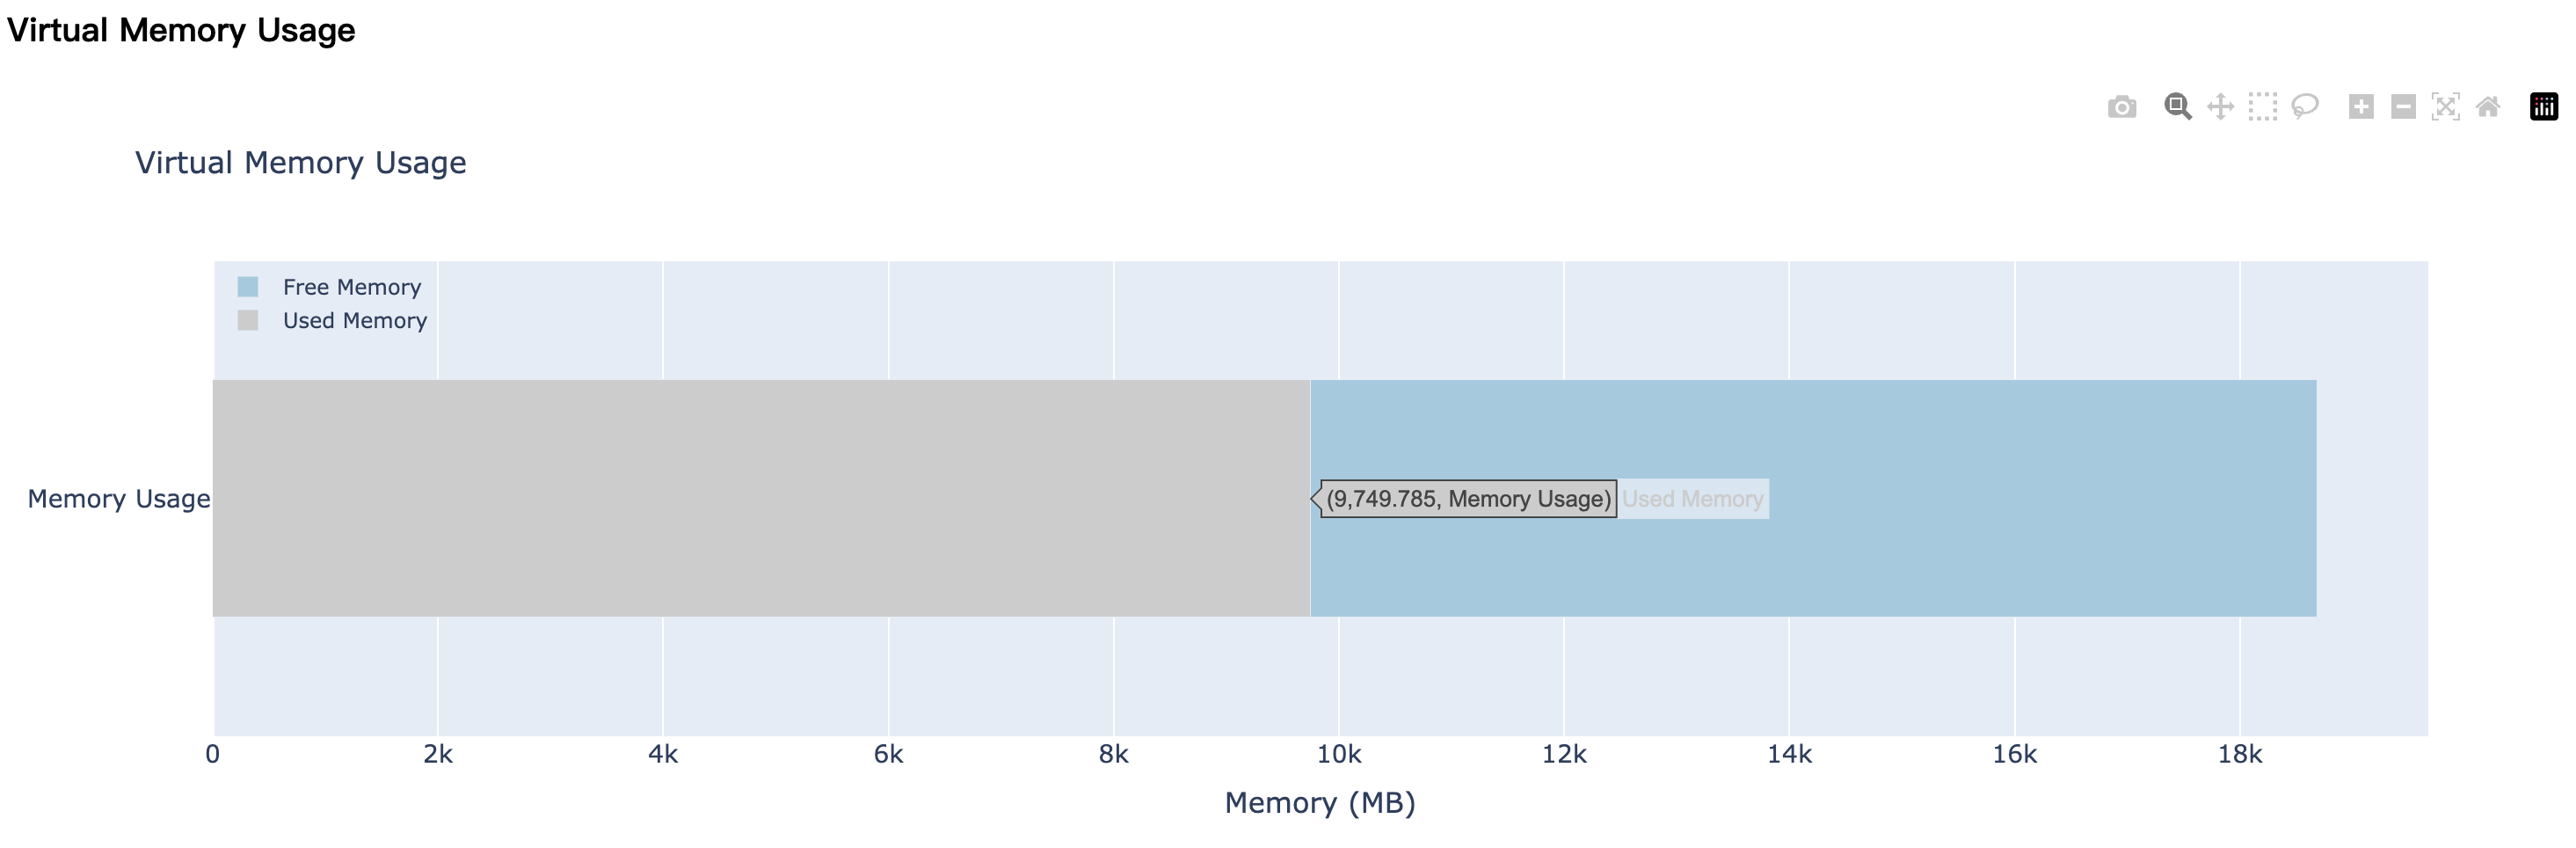
\includegraphics[width=0.95\textwidth]{figures/virtual-memory.png}
    \caption{Virtual Memory Usage}
    \label{fig:virtual-memory}
\end{figure}

Figure \ref{fig:virtual-memory} shows the used and free virtual memory. 

\begin{figure}[!htbp]
    \centering
    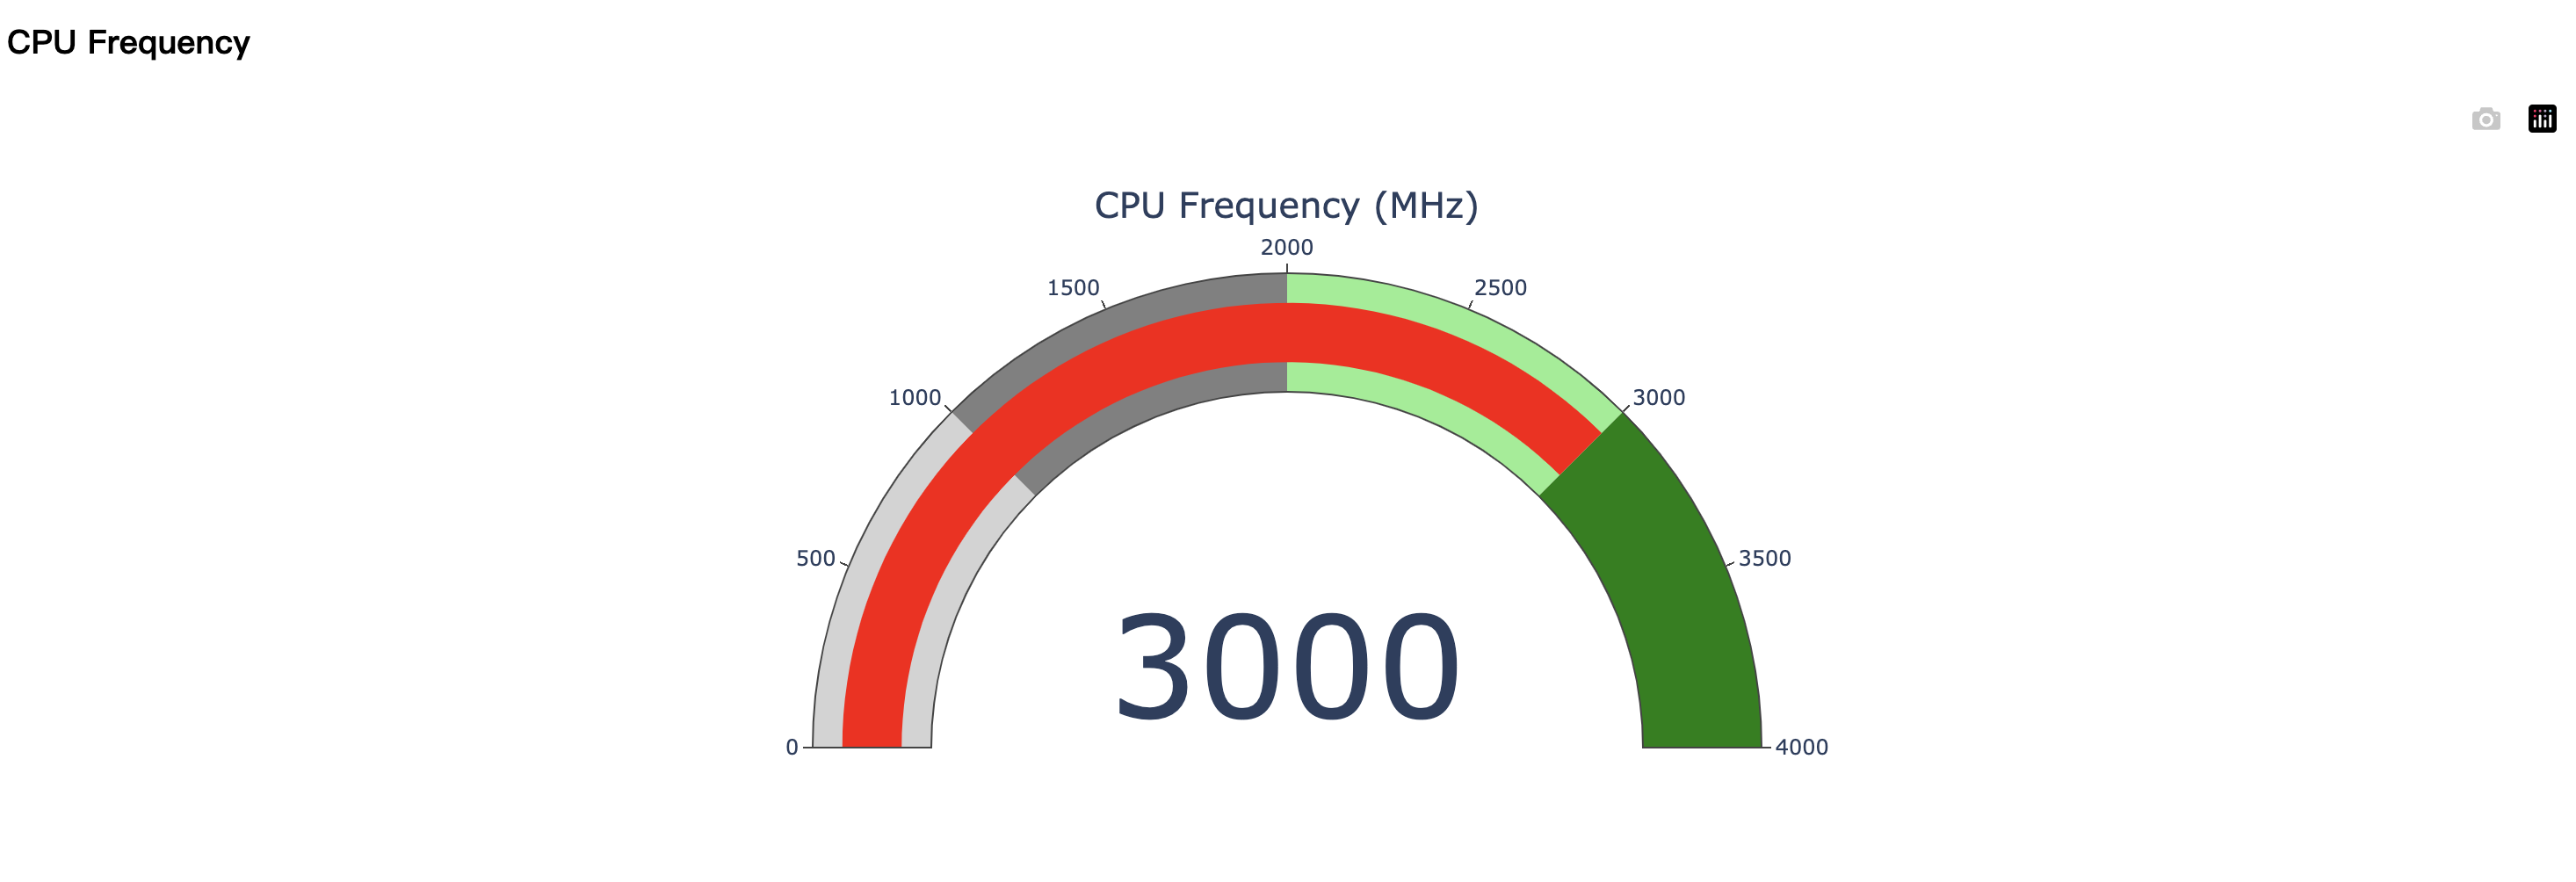
\includegraphics[width=0.95\textwidth]{figures/cpu-freq.png}
    \caption{CPU Frequency}
    \label{fig:cpu-freq}
\end{figure}

\newpage

Figure \ref{fig:cpu-freq} shows the current CPU speed. 

\begin{figure}[!htbp]
    \centering
    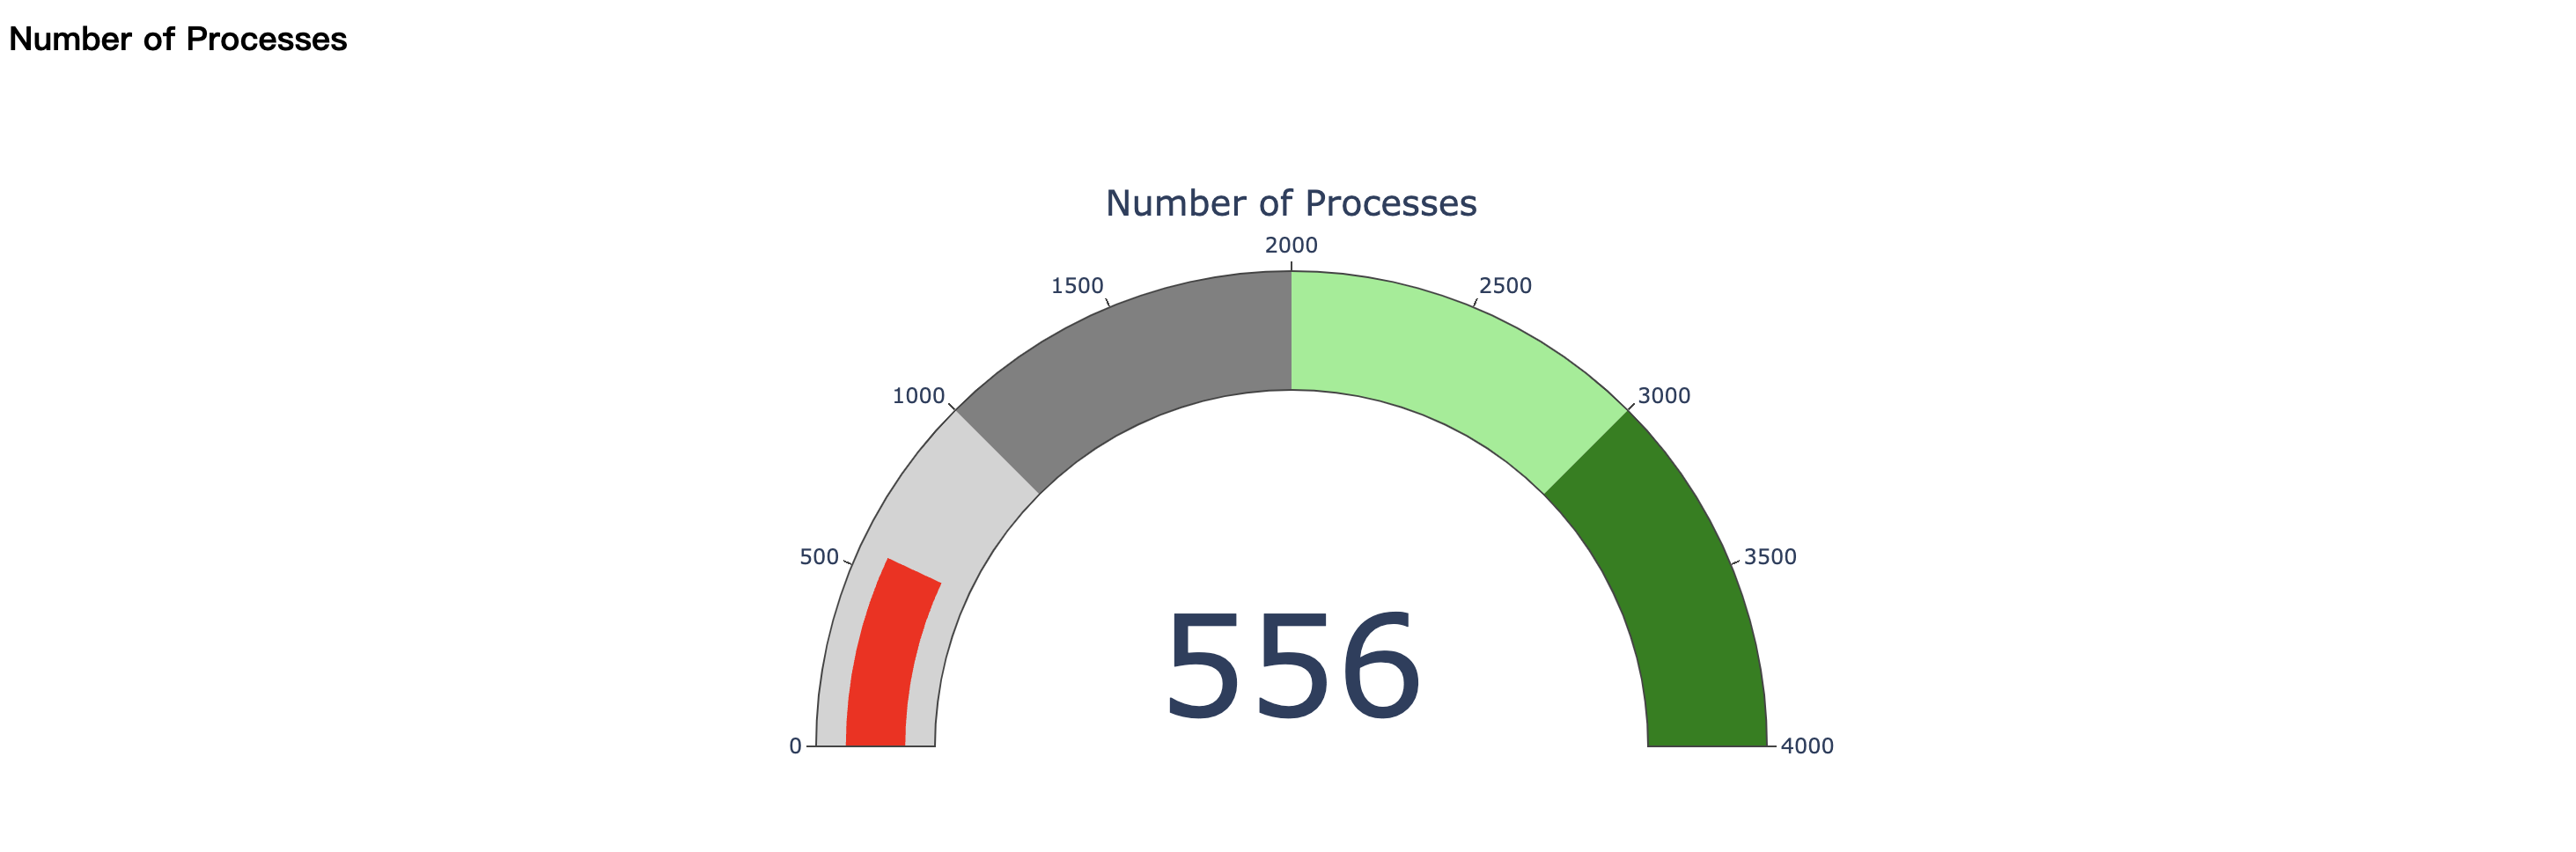
\includegraphics[width=0.95\textwidth]{figures/n-pids.png}
    \caption{Number of Processes}
    \label{fig:n-pids}
\end{figure}

Figure \ref{fig:n-pids} shows the current number of processes.

\end{document}